\section{Nebulas Rank}
\label{sec:rank}

\subsection{Nebulas Rank Overview} \label{subsec:value}
Currently the Blockchain technology and community have grown into a large scale ecosystem. However, people's perception of Blockchain world is still relatively flat; there is no reasonable way to evaluate the entity, such as user's address, on the blockchain yet. Therefore, we try to come up with a universal value measurement. By mining activities occurs on chain, the value of every entity (address) is able to be quantified as \textbf{Nebulas Rank}. \textbf{Nebulas Rank} is aimed at two goals:
\begin{itemize}
	\item As a native value measurement, \textbf{Nebulas Rank} could become core algorithms for many fundamental scenarios, such as consensus (see \refsec{}), DIP (see \refsec{}) and Blockchain search engine (see \refsec{}), etc.
	\item \textbf{Nebulas Rank} could inspire various value measurements, as well as deeper insights into the blockchain ecosystem.
\end{itemize}
Based on the goals above, we define the value measurement of \textbf{Nebulas Rank} to be three-fold:
\begin{itemize}
	\item Liquidity, the frequency and scale of transactions, is the first dimension that \textbf{Nebulas Rank} considers. Essentially, by means of capital liquidity, financial activity can promote efficient configuration of social resources and promote economy development. Blockchain established a value network. Thus more transactions and larger transaction scale produce better liquidity, and better liquidity further increases more transactions and larger transaction scale, forming a complete mechanism of positive feedback.
	\item Propagation, the scope and depth of liquidity, is the second dimension that \textbf{Nebulas Rank} considers. In social network, the propagation property, i.e. speed, scope and depth of information propagation, is key measurement indicating network quality and users growth. We see same pattern in the Blockchain world. Better propagation means wider and deeper assets liquidity, which improves the quality of assets in the Blockchain world, and increases the scale of assets.
	\item Interoperability is the third dimension that \textbf{Nebulas Rank} considers. During the early stage of Internet, there were just simple websites and isolated information. Nowadays, all kinds of Internet platforms begin to interact with each other and the small information islands begin to disappear. This tendency could be understood as a process of recognizing information from higher dimensional perspective. We believe that Blockchain world also follows the same roadmap, whose development will be faster. There will be more information of users' assets, smart contract and DApp. And also, there will be more frequent interactions among them. Thus better interoperability will become more important.
\end{itemize}

We choose transaction records on chain as source data for \textbf{Nebulas Rank}. Because comparing with real world, the "trajectory" in Blockchain world is more clear and trustworthy: the transaction data on chain loyally records every transferring among addresses and invoking of "smart contracts". But it is not trivial to design rank algorithm for Blockchain transaction data, since comparing with real world, the transactions in Blockchain world are naturally anonymous and bears larger data scale. So we depict three properties for \textbf{Nebulas Rank}:
\begin{itemize}
	\item Truthful. An entity must pay reasonable effort to improve its rank, which assures that the algorithm can identify trusted valuable users. On one hand, in scenarios like consensus and DIP, truthful ranking encourages users to contribute truthfully in order to realize positive feedback. On the other hand, truthful result provides meaningful hierarchy representation of all users, which will be more helpful for decision makers;
	\item Computable. As a fundamental field, \textbf{Nebulas Rank} of every user should be accessible instantly and thus requires low computational complexity;  
	\item Reproducible. Due to consensus and DIP, the running result of \textbf{Nebulas Rank} algorithm needs to be identical by any client.
\end{itemize}

Next we design basic framework of \textbf{Nebulas Rank}. First, transaction records are represented in the form of graph. By the definition of transaction graph (entity graph), every node is mapped to one entity, and each edge represents the transferring between two entities\cite{Tschorsch2015}. Transaction graph embeds the fact that money transferring among users leads to assets flowing, which helps to represent the concepts of liquidity and propagation defined before. Meanwhile, the form of graph is convenient to formulate the interoperability among contracts. With the derived transaction graph, we rank nodes by their network centrality. In the scenario of \textbf{Nebulas Rank}, LeaderRank\cite{Chen2013}\cite{Li2014} is a more reasonable measurement and outperforms PageRank and NEM\cite{nem}.。

\subsection{Transaction Graph} \label{subsec:txg}
This subsection introduces how to derive transaction graph from transaction history.

First, we take effective transferring among  individual addresses during the past $T$ (generally $T$ is the number of blocks in a month) blocks, denoted by $T_{xs}$:
\begin{align}
T_{xs} = \{(s,t,\tau, a)| \tau = \#CurrentBlock-T \dots \#CurrentBlock \land a > 0 \}
\end{align}
, where $s$, $t$ and $a$ are source address, target address and transfer amount.

Then based on $T_{xs}$, a directed weighted simple graph is constructed, denoted as $G=(V, E, W)$, where node set, edge set and edge weights are denoted by $V$, $E$ and $W$ respectively. Additionally, let $N = |V|$,$M = |E|$. For simplicity, every node is represented by an integer between $1$ and $N$.

Every node represents an individual account's address, and each edge represents the intensity between two addresses. Edges are directed and are assigned with weight $w_e$ aggregating top $K$ amounts of all related transactions:
\begin{align}\label{formula:edgeweight}
w_e = \sum_{i=1}^K a_i, s.t. a_i \in \{a|(s,t,\tau,a) \in T_{xs} \} \land a_1 \geq a_2 \dots
\end{align}

\begin{figure}[h]
\centering
	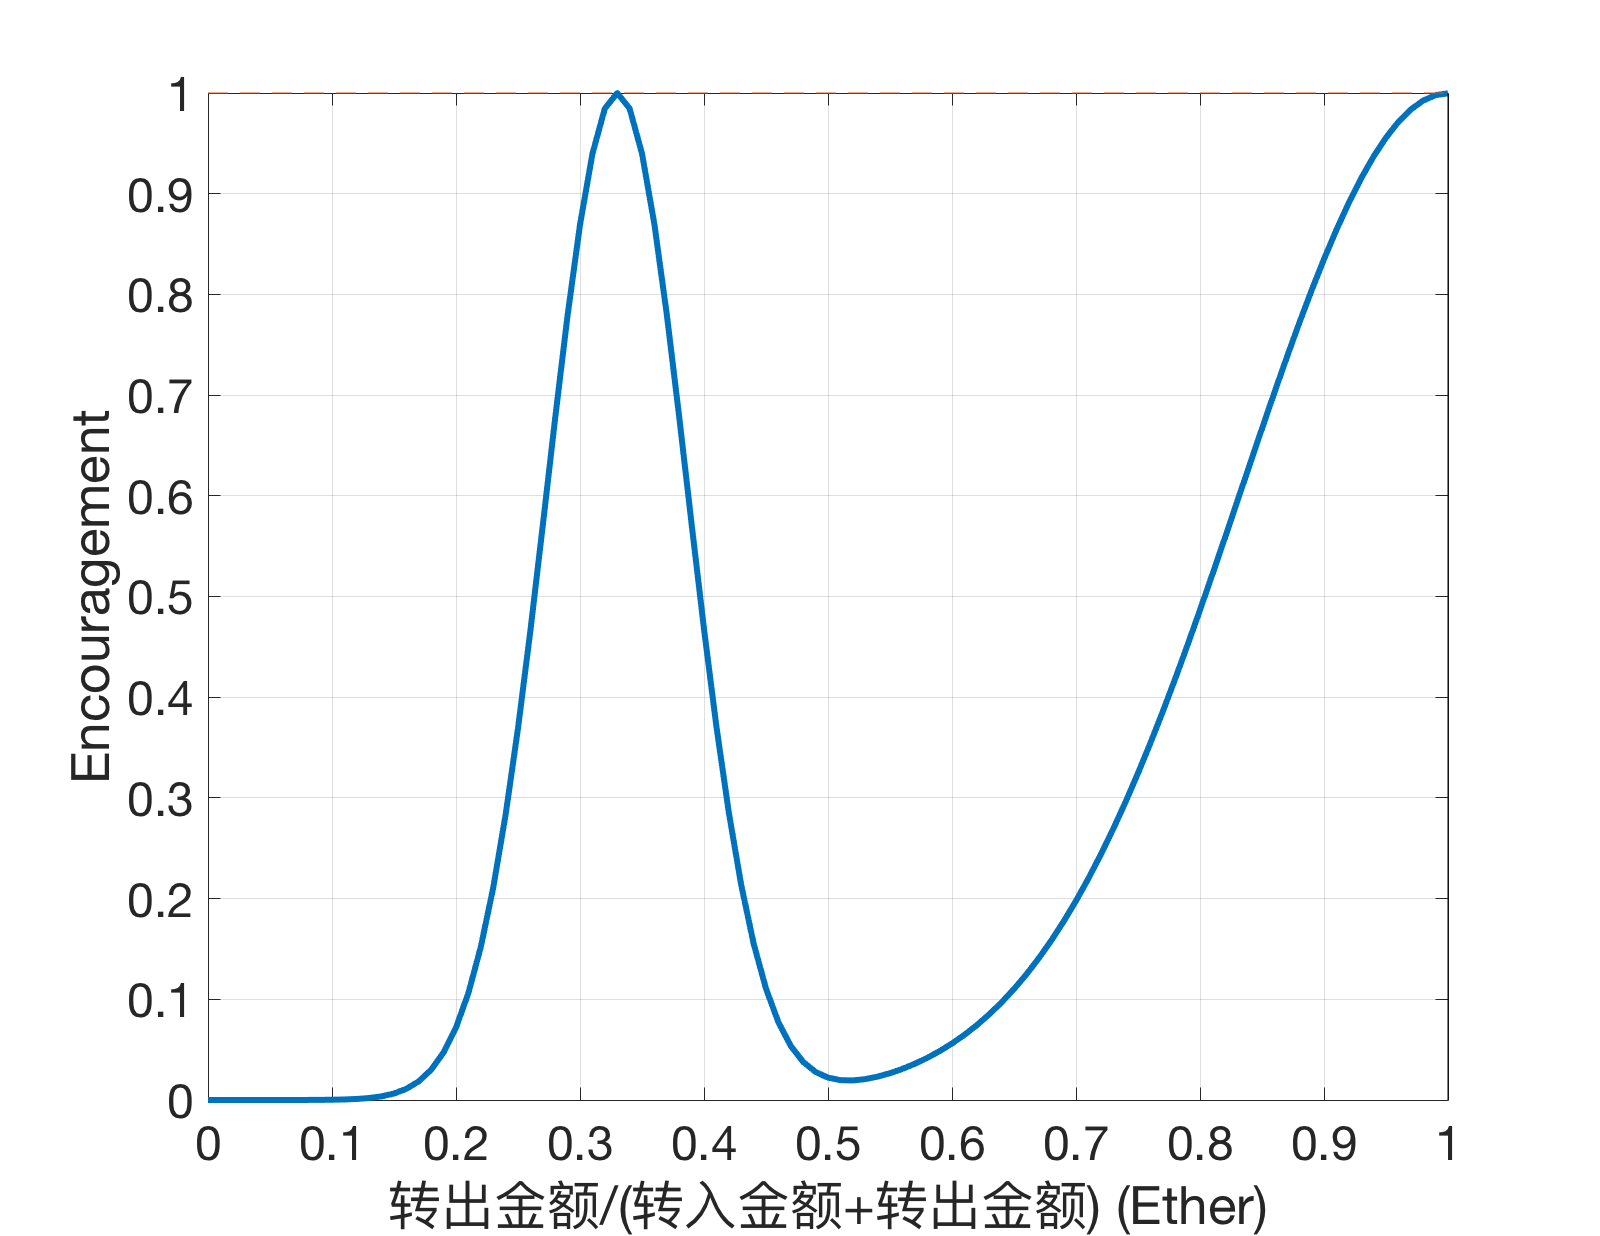
\includegraphics[width=0.55\textwidth]{figs/encouragement.png}
	\caption{Encouragement Function}\label{fig:encouragement}
\end{figure}

Then for each node, according to its in-transfers and out-transfers during the past $T$ blocks, we compute its "coinage", denoted by $C_v$; also, based on an "encouragement function" shown in \reffig{fig:encouragement}, we compute its encouraged value, denoted by $E_v$.\footnote{Encouragement function can be represented as a linear combination of two normal distributions, which outputs peak value when the money transferred out is zero or of some ratio of the amount transferred in.} And then the edges' weight is reduced by their target node's $C_v$ and $E_v$.

Finally, we take the largest weakly connected component of the whole graph, only remaining nodes belonging to this component.

The graph derivation described above contributes to the "truthful" property defined at \refsec{subsec:value}, the evidence of which is shown in \refsec{subsec:robust}.

We collect data on Ethereum Main Net Blockchain. It starts at \#3629091(roughly on May 1st, 2017) and ends at\#3800775(roughly on May 31st, 2017), containing $171,684$ transactions in total. Let $T=171,684$, $K=2$, we construct the transaction graph according to the method introduced by this subsection, and its visualization is shown as \reffig{fig:wgc}. Some nodes are labeled by tags in Etherscan\cite{etherscan}, and all nodes are resized by their degree. It could be observed that some famous exchanges usually interacts with more accounts than others. Besides, the identities of some addresses who contributes a lot transactions still remains unknown. 

\begin{figure}[h]
	\centering
	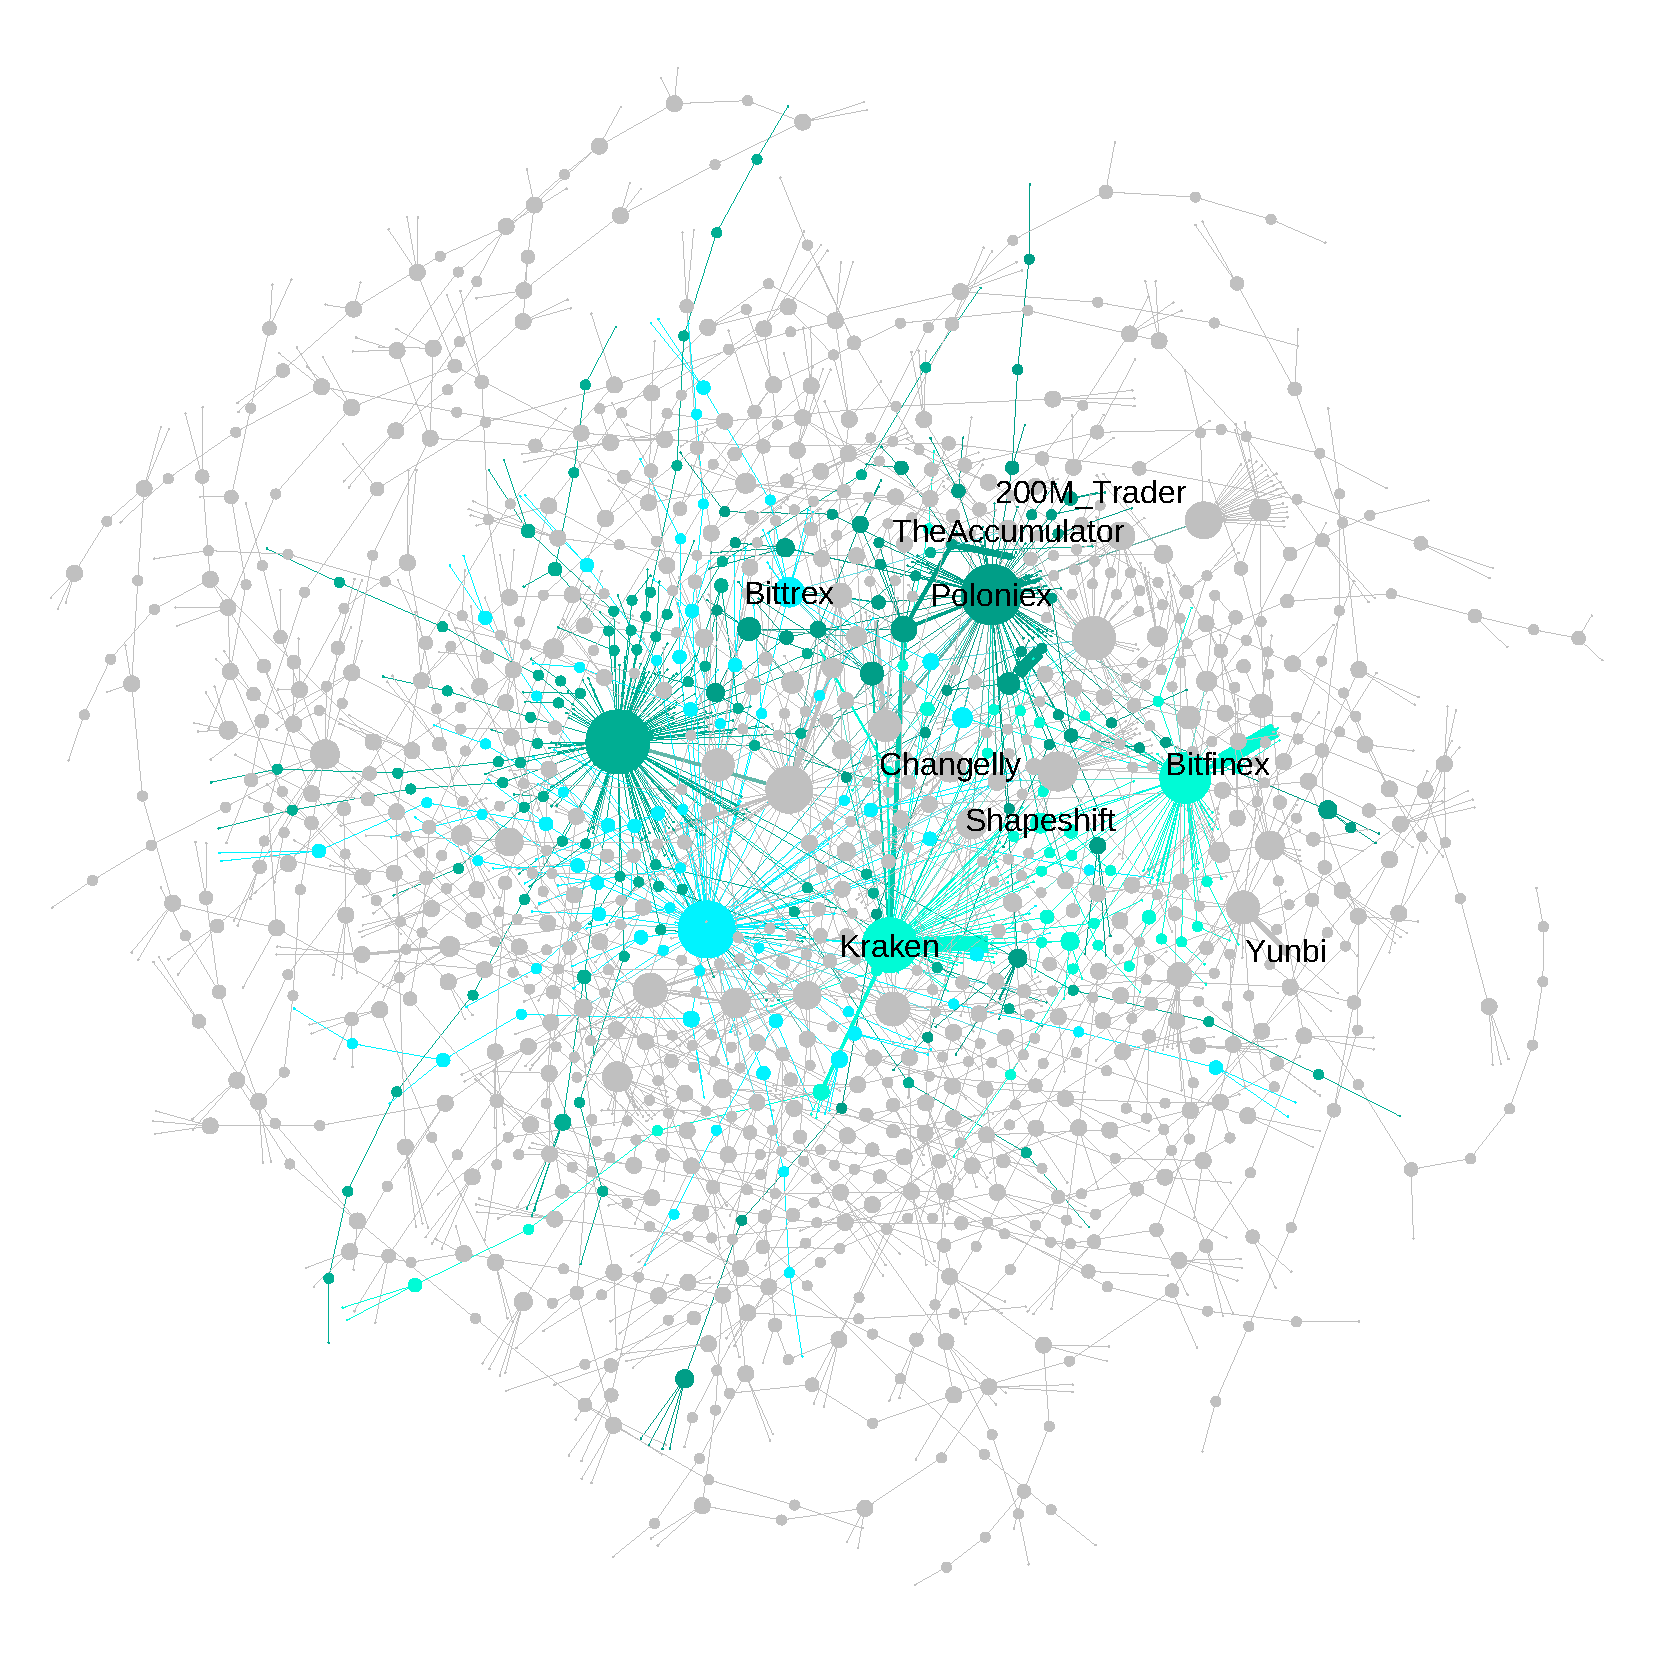
\includegraphics[width=0.85\textwidth]{figs/wgc1.png}
	\caption{Transaction Graph (Partly) Visulazation }\label{fig:wgc}
\end{figure}

\subsection{Ranking Algorithm} \label{subsec:leaderrank}
This subsection introduces how to rank nodes by their importance in the derived transaction graph.

We adopt LeaderRank\cite{Chen2013}\cite{Li2014} as the main method. First, a ground node is added into the transaction graph, denoted by $\mathcal{G}$ and numbered as $N+1$. Then we establish double link between the ground node and every other node, weighting by the following formula:
\begin{align}\label{formula:weight1}
	\forall v \in V, w_{(v, \mathcal{G})} = \alpha A_v
\end{align}
\begin{align}\label{formula:weight2}
\forall v \in V,  w_{(\mathcal{G}, v)} = \beta B_v
\end{align}
, where 
\begin{align}
	\forall v \in V, A_v = \{ \sum_{(u,v)\in E} w_{(u,v)} - \sum_{(v,u) \in E} w_{(v, u)}, 0 \} + \lambda C
\end{align}
\begin{align} \label{formula:b}
\forall v \in V,  B_v =  \sum_{(u,v) \in E} w_{(u,v)} + \mu C
\end{align}
\begin{align}
	C = median\{w_e| e \in E\}
\end{align}

$\alpha, \beta, \mu, \lambda$ are parameters. The weighting scheme can be understood as that, nodes with more in-degree receive more in-link from the ground node; nodes with more absolute income, i.e. in-degree minus out-degree, outputs stronger link into the ground node. 

The running process of LeaderRank is similar with PageRank, which could be understood as computing the convergence state of a Markov process. What is different is that, after adding the ground node, it does not need to consider the damping factor of PageRank\cite{Brin2010}\cite{page1999pagerank} any more.

LeaderRank的计算过程和PageRank基本相同,可以理解为求马可夫链的稳定状态。所不同的是,添加了Ground节点之后,不再需要考虑PageRank的damping factor\cite{Brin2010}\cite{page1999pagerank}。即按(\ref{formula:matrix})构造矩阵$H$后,进行如(\ref{formula:iteration})所示的迭代(初始值设置见(\ref{formula:init})),直至收敛为止,最后去掉Ground节点的评分即为交易图各点重要程度得分。

\begin{align} \label{formula:iteration}
	P^{t+1} = H \times R^{t}; P^1=[\frac{1}{N}, \frac{1}{N}, \dots, \frac{1}{N}, 0]^T
\end{align}
\begin{align} \label{formula:matrix}
	h_{ij} = \frac{w_{(j,i)}}{\sum_k w_{(j,k)}}
\end{align}
\begin{align} \label{formula:init}
\forall v \in V, P^*_v \leftarrow P^*_v + \frac{P^*_{\mathcal{G}}}{N}
\end{align}


我们认为,LeaderRank可以较好地满足\refsec{subsec:value}定义的价值尺度和算法性质:
\begin{itemize}
	\item LeaderRank可以理解为在资金流动网络动态平衡状态下通过每点的流量,这契合了\textbf{Nebulas Rank}的『流动性』、『传播性』和『互操作性』等尺度;
	\item (\ref{formula:weight2})和(\ref{formula:b})所定义的赋权机制可以加大攻击难度(见\refsec{subsec:robust}的讨论),更好地满足『可信』性质;
	\item LeaderRank的计算可以用迭代方式完成,由于网络的稀疏性(见\refsec{subsec:txg}的结果),矩阵运算复杂度不高,能够满足『可计算』和『可复现』的性质。
\end{itemize}


\\label{subsec:robust}

可信性,即抵抗操纵的能力,是\textbf{Nebulas Rank}最重要同时也是最具挑战的目标。部分恶意操纵的手段有以下几种:
\begin{itemize}
	\item 环形转账,攻击者沿环形拓扑,让同一笔资金不断流过对应的边,以提高边权;
	\item 频繁同权威交易所账户交易,多次在交易所账户中取入取出同一笔资金,获得较好的网络结构位置;
	\item 向其他任意账户转钱,提高出度,并且提高资金流出的传播性;
	\item 控制多个账户形成独立分支,伪造中心节点;
\end{itemize}

\textbf{Nebulas Rank}通过以下几个机制,可以弱化操纵效果:
\begin{itemize}
	\item 由于设置了$T$个区块的滑动时间窗,攻击者无法在短期内迅速提高自己的排名;
	\item 因为边权由最高的几次交易金额决定,在一个环状拓扑内的多次转账不能无限提高各边权值,同时,从\refsec{subsec:txg}采集的数据看,有$91\%$的双方只进行了一或两次交易,因此$K$取$2$可以最大限度保留边的强度信息,同时抵抗环形转账攻击;
	\item 为了获得更高『币龄』,用户需要让资金在自己的账户内『停留』一段时间,进而拖慢攻击者的交易速度;
	\item 为了获得最大的『鼓励值』,如\reffig{fig:encouragement}所示,账户需要在当前周期内储蓄全部收入,或者只转出少于收入一半的金额,因此伪造资金流动时,攻击者的本金会因各个账户的储蓄效应而迅速衰减;
	\item 由于取了最大弱联通分支,伪造的独立分支会被视为噪声而过滤清除。从\refsec{subsec:txg}采集的数据看,交易图有$453,285$个节点,$970,577$条边,有$1,169$个弱分支,其中最大弱分支有$449,746$个节点,占全体节点的$99.2\%$,次大弱分支有$133$个节点,仅占全体节点的$0.03\%$,因此取最大联通分支可以最大限度保留网络正常成分并且过滤噪声数据;
	\item 相对于PageRank和NCDawareRank\cite{Nikolakopoulos2013}等网页排序算法,(\ref{formula:weight2})和(\ref{formula:b})所定义的赋权机制对低入度的节点评分偏向『保守』,即低入度的节点获得来自Ground节点的链接更弱。在区块链交易图中,低收入节点更容易被伪造,而频繁向其他任意地址转账并不能提高收入,因此使用\textbf{Nebulas Rank}的方法可以提升操纵难度;
\end{itemize}

接下来,基于2017年5月份Ethereum的交易图(见\refsec{subsec:txg}),我们展示一系列结论。

首先,我们列出\textbf{Nebulas Rank}排名部分地址,如表\ref{table:nr}所示\footnote{备注来源: Etherscan\cite{etherscan}}, 交易所账户以及部分交易吞吐量较大地址的排名靠前。

\newpage

\begin{table}[!htbp]
\centering
\caption{\textbf{Nebulas Rank}排名前$10$名及部分其他地址}
\label{table:nr}
\begin{tabular}{llllll}\toprule
排名 & 地址                                                                                    & Nebulas Rank & 备注          & 转出金额(Ether) & 转入金额(Ether) \\
1  & \begin{tabular}[c]{@{}l@{}}0x267be1c1d684f78cb4f\\ 6a176c4911b741e4ffdc0\end{tabular} & 0.449275     & Kraken\_4   & 3214232.06  & 350008.00   \\
2  & \begin{tabular}[c]{@{}l@{}}0xd4c5867cec094721aab\\ c3c4d0fd2f2ac7878c79a\end{tabular} & 0.093798     &             & 58000.00    & 100947.00   \\
3  & \begin{tabular}[c]{@{}l@{}}0x027beefcbad782faf69f\\ ad12dee97ed894c68549\end{tabular} & 0.049277     & QuadrigaCX  & 207440.11   & 65606.40    \\
4  & \begin{tabular}[c]{@{}l@{}}0x0ee4e2d09aec35bdf08\\ 083b649033ac0a41aa75e\end{tabular} & 0.046831     &             & 56465.00    & 60087.96    \\
5  & \begin{tabular}[c]{@{}l@{}}0xc257274276a4e539741\\ ca11b590b9447b26a8051\end{tabular} & 0.037628     &             & 1071105.93  & 1434106.72  \\
6  & \begin{tabular}[c]{@{}l@{}}0xa53e0ca7d246a764993\\ f010d1fde4ad01189f4e6\end{tabular} & 0.033488     &             & 7764.68     & 3201.00     \\
7  & \begin{tabular}[c]{@{}l@{}}0xf259e51f791e9ed26e8\\ 9b6cae4a7c6296bfbd0b8\end{tabular} & 0.033481     &             & 3307.00     & 7731.30     \\
8  & \begin{tabular}[c]{@{}l@{}}0xf195cac8452bcbc836a\\ 4d32cfb22235af4ac1e9c\end{tabular} & 0.026343     &             & 10863.87    & 2315.69     \\
9  & \begin{tabular}[c]{@{}l@{}}0x94435d12c51e19d5b5c\\ 8656763f9069d37791a1a\end{tabular} & 0.024970     &             & 12938.58    & 15858.90    \\
10 & \begin{tabular}[c]{@{}l@{}}0x7580ba923c01783115d\\ 79975d6a41b3d38eff8d5\end{tabular} & 0.021670     &             & 263000.00   & 364793.49   \\
16 & \begin{tabular}[c]{@{}l@{}}0xcafb10ee663f465f9d10\\ 588ac44ed20ed608c11e\end{tabular} & 0.004995     & Bitfinex\_1 & 360000.00   & 1435858.40  \\
51 & \begin{tabular}[c]{@{}l@{}}0xd94c9ff168dc6aebf9b\\ 6cc86deff54f3fb0afc33\end{tabular} & 0.000868     & yunbi\_1    & 1179224.74  & 1202539.53  \\
64 & \begin{tabular}[c]{@{}l@{}}0x70faa28a6b8d6829a4b\\ 1e649d26ec9a2a39ba413\end{tabular} & 0.000590     & Shapeshift  & 52501.81    & 651933.49   \\
\bottomrule
\end{tabular}
\end{table}

接着,对比交易金额和\textbf{Nebulas Rank}的关系。由于区块链交易可以理解为『资金交换』类型的网络流,根据\textcite{Borgatti2005}的研究工作,节点的度,即邻接边权值之和,是适用于此类网络的一个合适的中心性测度。以每个节点为中心思考,度,即交易金额(转入转出金额的和),是节点一跳局部信息的体现,直接反映了对应地址的历史资金流量,因此应该作为衡量排序算法的基准。交易金额与\textbf{Nebulas Rank}的关系如\reffig{fig:nrio}所示:没有节点能够以较低的交易金额获取靠前排名,而交易金额较大的节点也要满足一定条件才能取得高的排名,这可以大致印证\textbf{Nebulas Rank}的可信性。

\begin{figure}[!htbp]
	\centering
	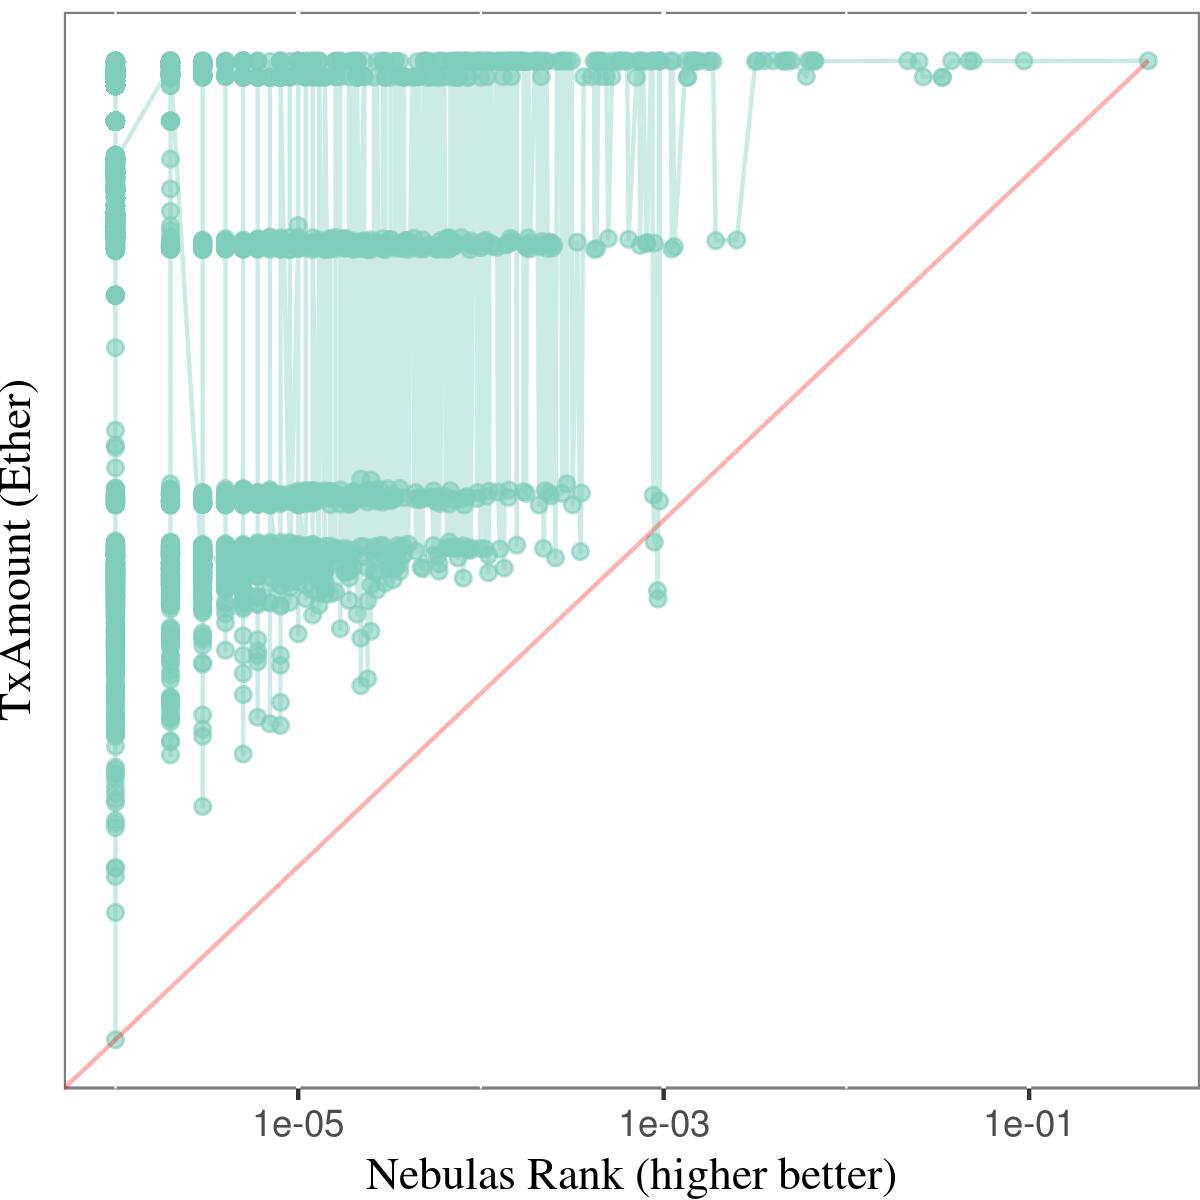
\includegraphics[width=0.40\textwidth]{figs/MAY_lr.png}
	\caption{Nebulas Rank v.s. 交易金额}\label{fig:nrio}
	\caption*{\footnotesize{横坐标为Rank值,纵坐标为交易金额,均为对数形式}}
\end{figure}


最后,我们仿真一类特定的攻击,攻击者选定某权威交易所节点,在排名计算周期内创造$X$次环形交易,每次交易时,攻击者先经由某新建地址向交易所节点转入$Y$Ether,之后经另一新建节点从交易所节点取出$Y$Ether,攻击方式示意图如\reffig{fig:loop}所示。

\begin{figure}[!htbp]
	\centering
	%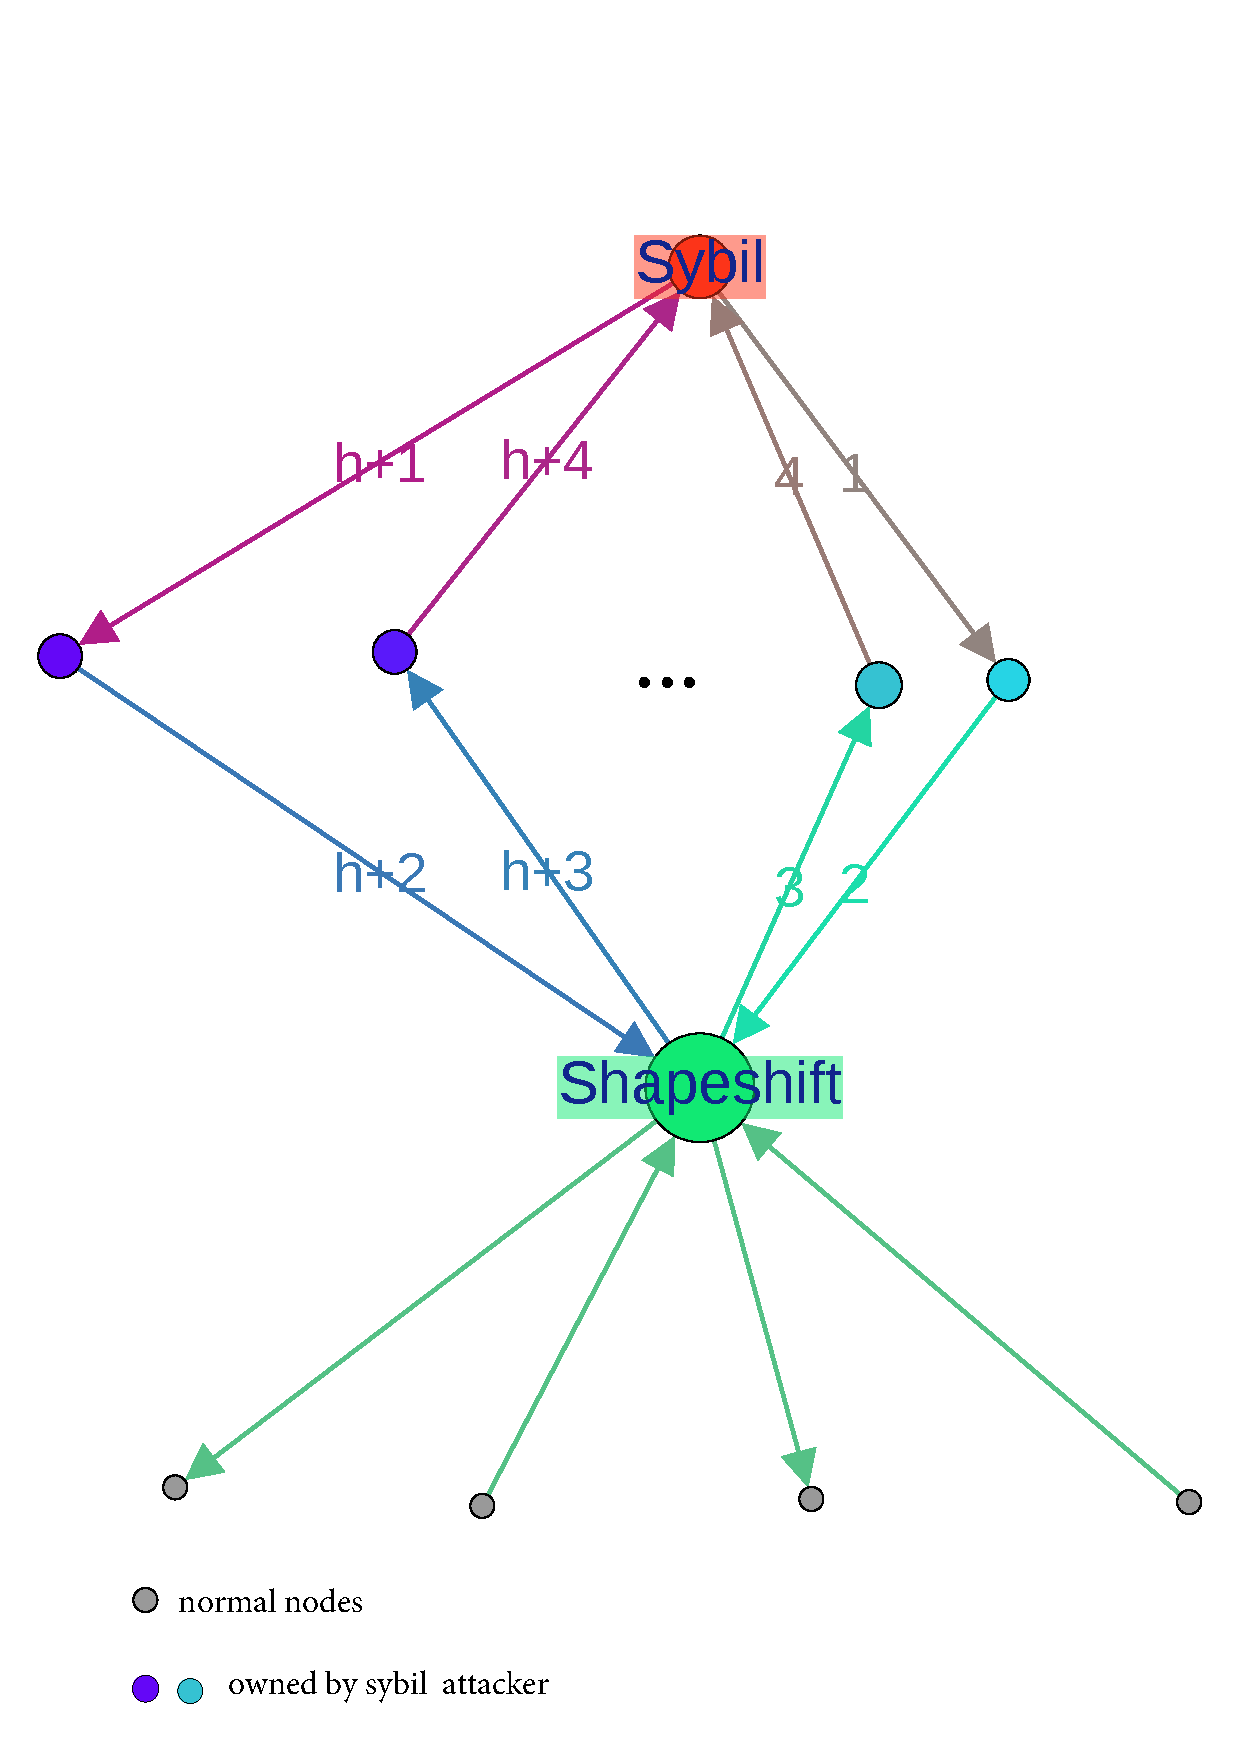
\includegraphics[width=0.35\textwidth]{figs/attack.pdf}
  \begin{tikzpicture}
  \pgfmathsetmacro{\YMD}{2}
  \pgfmathsetmacro{\XMD}{1.5}
\tikzset{
  hnode/.style={draw, circle, on grid, align=center, minimum height=2ex},
  base/.style={draw, circle, on grid, align=center, minimum height=4ex},
  sybil/.style={draw, circle, on grid, align=center, minimum height=4ex, fill=blue!20},
  normal/.style={draw, circle, on grid, align=center, minimum height=1ex, fill=gray!20},
  coord/.style={coordinate, on grid, node distance=6mm and 25mm},
}
%
\tikzset{>=stealth',
  every join/.style={->}, very thick}

       \node [base, fill=green!=20] (ss) at (0, 0) {} node[right
       = 1ex of ss] {Shapeshfit};

       \node (dot) at ($(ss.north) + (0, \YMD)$) {...};

       \node [sybil] (sy) at ($(dot.north) + (0, \YMD)$) {} node[right=1ex of
       sy]{Sybil};

       \node [hnode, fill=brown!50] (hh4) at($(dot.west) + (-\XMD, 0)$){};
       \node [hnode, fill=brown!50] (hh1) at ($(hh4.west) + (-\XMD, 0)$){};

       \node [hnode, fill=cyan!20] (h4) at ($(dot.east) + (\XMD, 0)$){};
       \node [hnode, fill=cyan!20] (h1) at ($(h4.east) + (\XMD, 0)$){} node
       [right = 1ex of h1]{owned by sybil attacker};

       \node [coord] (c) at($(ss.south) + (0, -\YMD)$) {};

       \node [normal] (n2) at ($(c.west) + (-\XMD, 0)$){};
       \node [normal] (n1) at ($(n2.west) + (-\XMD, 0)$){};
       \node [normal] (n3) at ($(c.east) + (\XMD, 0)$){};
       \node [normal] (n4) at ($(n3.east) + (\XMD, 0)$){} node [right=1ex of
       n4] {normal nodes};

       \draw[->, color=red] (sy) -- (hh1) node [midway, left]{h+1};
       \draw[->, color=red] (hh4) -- (sy) node [midway, right]{h+4};
       \draw[->, color=olive] (h4) -- (sy) node [midway, left]{4};
       \draw[->, color=olive] (sy) -- (h1) node [midway, right]{1};

       \draw[->, color=red] (hh1) -- (ss) node [midway, left]{h+2};
       \draw[->, color=red] (ss) -- (hh4) node [midway, right]{h+3};
       \draw[->, color=olive] (ss) -- (h4) node [midway, left] {3};
       \draw[->, color=olive] (h1) -- (ss) node [midway, right]{2};

       \draw[->] (ss) -- (n1);
       \draw[->] (n2) -- (ss);
       \draw[->] (ss) -- (n3);
       \draw[->] (n4) -- (ss);

\end{tikzpicture}

	\caption{将交易所纳入环形交易的攻击示意图}\label{fig:loop}
\end{figure}

测试选择的交易所为Shapeshift (0x70faa28a6b8d6829a4b1e649d26ec9a2a39ba413),结果如\reffig{fig:antiManipulation}所示:随着攻击者投入本金提高,使用任何算法的情况下,其收益都会越来越高,但是使用\refsec{subsec:txg}所述的方式构造交易图方式可以使得攻击效果显著减弱,并且\textbf{Nebulas Rank}可以既充分重视高交易量地址,又一定程度抵抗攻击。

\begin{figure}[!htbp]
	\centering
	%\subfigure[]{}
	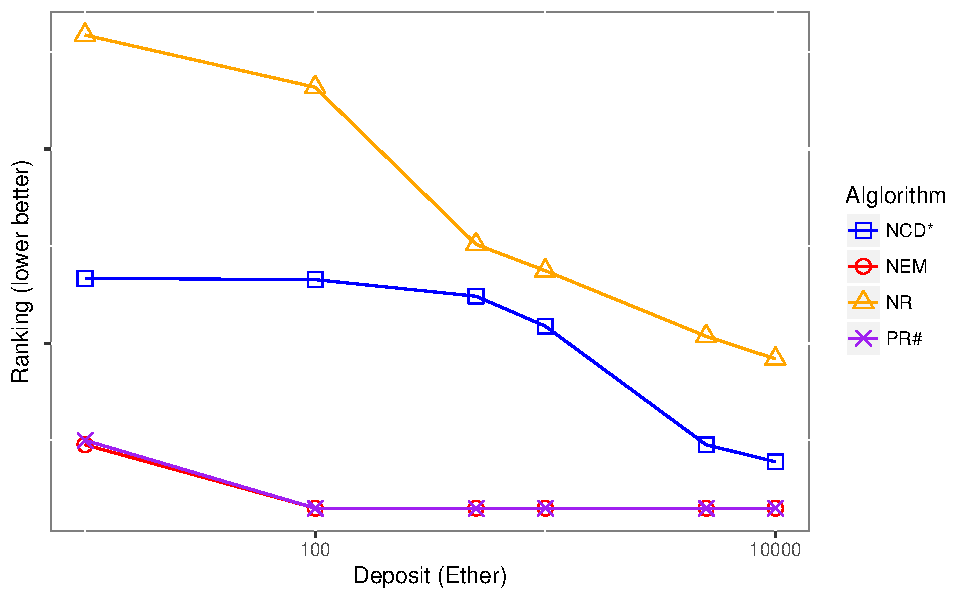
\includegraphics[width=0.7\textwidth]{figs/AttackDeposit.pdf}
	%\label{subfig:deposit}}
	%\subfigure[攻击投入本金$\Xi5000$, 攻击次数对排名的影响]{ 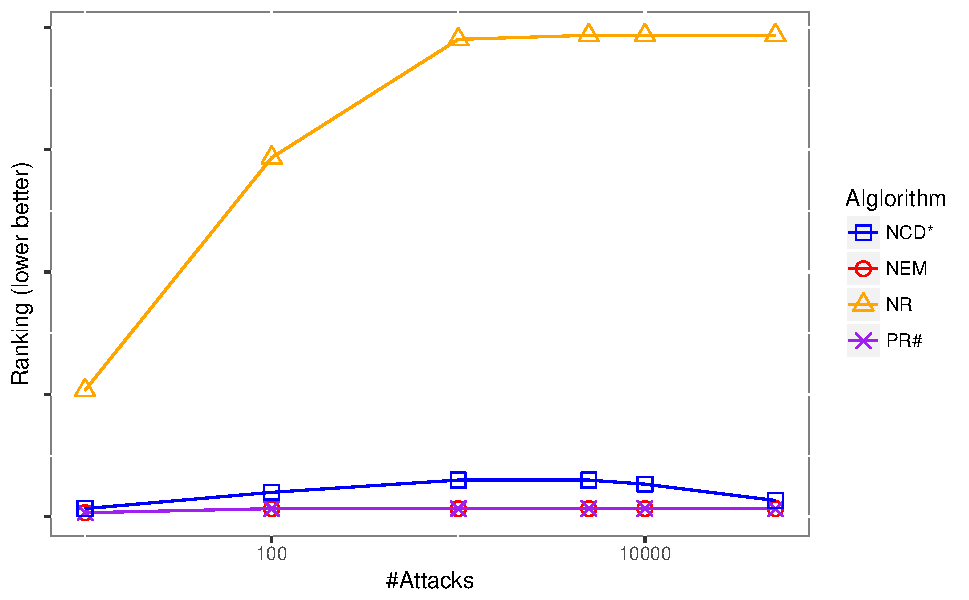
\includegraphics[width=0.7\textwidth]{figs/AttackTimes.pdf} \label{subfig:times}}
	\caption{抗操纵测试结果 }
	\label{fig:antiManipulation}
	\caption*{\footnotesize{攻击次数固定为5000次, 攻击投入本金对排名的影响 \\ 横轴为攻击成本,纵轴为效果排名(越靠前坐标值越小),均为对数坐标 \\
	NR:交易图如\refsec{subsec:txg}所述,排序算法按照\refsec{subsec:leaderrank}所述;\\PR$^*$:交易图如\refsec{subsec:txg}所述,PageRank排序算法;\\ NCD$^*$:交易图如\refsec{subsec:txg}所述,NCDawareRank排序算法;\\ NCD$^{\#}$:交易图如\cite{nem}所述,NCDawareRank排序算法;\\ PR$^{\#}$:交易图如\cite{nem}所述,PageRank排序算法 \\ PageRank的damping factor为0.15;NCDawareRank使用pscan\cite{chang2017mathsf}社群划分算法,$\eta=0.75$, $\mu=0.1$}}
\end{figure}

\subsection{Related Works} \label{subsec:related}
中心性,作为最核心的节点排序指标,是过去几十年网络科学领域研究最多的一个概念\cite{newman2010networks}。丰富的文献引入了大量中心性测度,包括度中心性\cite{freeman1979set}, 特征值中心性\cite{bonacich1972factoring}, Katz中心性\cite{katz1953new}, 接近度中心性\cite{sabidussi1966centrality}, 介数中心性\cite{freeman1977set}\cite{freeman1978centrality}\cite{freeman1991centrality}\cite{noh2004random}\cite{newman2005measure}, PageRank\cite{Brin2010}, HITS\cite{kleinberg1999authoritative}, SALSA\cite{Science2001}, 等等。此外还有许多工作试图用统一的框架来对中心性测度作出清晰的分类和综述\cite{Borgatti2005}\cite{Borgatti2006}\cite{Lu2016}。在设计\textbf{Nebulas Rank}时,需要首先考察交易图的性质,然后再选用合适的中心性。\textcite{Borgatti2005}工作中提到的资金交换网络和区块链交易图最为相近,但是提到的相关算法,如流中心性\cite{freeman1991centrality} 和随机游走中心性(又称电流中心性)\cite{newman2005measure},复杂度过高,在区块链交易图的规模上不符合\textbf{Nebulas Rank}的『可计算』性质。

自从比特币\cite{Nakamoto2008}系统在2009年发布以来,研究者们对比特币交易图做了一些试验性和统计上的分析\cite{Ron}\cite{Haslhofer}\cite{NielKondor2014}\cite{Baumann2014}, 同时试图使用交易图的结构来讨论比特币的匿名性问题\cite{Meiklejohn2013}\cite{Ober2013}\cite{pham2016anomaly}\cite{Fleder2015}\cite{Ferrin2015}。 在其他加密货币出现并流行之后,交易图分析拓展到了其他的区块链系统\cite{Chang2017}\cite{Anderson2016}。 \textbf{Nebulas Rank}采用的交易图概念和这些研究中的大致相同,即\textcite{Tschorsch2015}所总结的『实体图』。即每个用户实体被映射为一个节点。而每条有向边则代表两个用户之间的交易强度。事实上,早在如比特币一样的区块链系统发明之前,学者们就尝试对银行和国际交易的金融网络进行研究\cite{propper2008towards}\cite{Boss2004}\cite{Serrano2007}\cite{Bech2008}\cite{Fagiolo2009}\cite{Morten2006}\cite{Boss2004a}\cite{Krempel2002}\cite{Serrano2003}。 和区块链交易图相比,这些早期研究的网络还包含了额外的借贷活动。并且这些网络的规模非常小。总之,现有研究几乎没有专门针对大规模区块链交易图提出排序方法。

和\textbf{Nebulas Rank}最相关的工作是 NEM\cite{nem}的Proof-of-Importance机制,它采用了 NCDawareRank\cite{Nikolakopoulos2013}作为排序算法。 NCDawareRank\cite{Nikolakopoulos2013}利用了网络拓扑的社群效应。Proof-of-Importance使用SCAN\cite{xu2007scan}\cite{shiokawa2015scan}\cite{chang2017mathsf}作为社群聚类算法。虽然社区结构在交易网络的确存在并且可以帮助应对欺诈节点,却无法保证同一个实体对应节点一定可以映射到相同社群,因此利用社区划分的结果会提供一定的可操纵空间。此外\textcite{Fleder2015}使用PageRank来帮助发现感兴趣的比特币地址并分析它们的活动,但他们的工作仍然将人工主观分析作为主要方法,PageRank只起到辅助作用,这也和\textbf{Nebulas Rank}的目标不符。我们采用的算法时LeaderRank\cite{Chen2013}\cite{Li2014}。 它是PageRank的一种拓展形式。在PageRank中,每个节点都有相同的随机跳转概率,LeaderRank是对跳转概率一种简单但有效的改进,通过在网络中添加Ground节点和加权的双向链接,可以使得不同节点具有不同的随机跳入和跳出概率。\textbf{Nebulas Rank}的加权机制部分参考了\textcite{Li2014}的设计,使得入度更大的点更有可能被随机跳转到达。通过添加LeaderRank算法中的Ground节点,可以取得更符合区块链场景的排序结果。


